As discussed in Chapter III, we are interested in measuring the differential conductance of samples versus a DC bias voltage. This is because the differential conductance of a normal sample is directly proportional to the \ac{DoS} of a material. To see this, let's start off by considering the contribution of a single carrier tunneling from our contact to the sample, we also must consider carriers tunneling from the sample to the contact:
\begin{align}
    i_{sample \rightarrow contact} = -2e\frac{2\pi}{\hbar}|M|^{2}\left(\rho_{s}\left(\varepsilon\right)\cdot f\left(\varepsilon\right)\right)\cdot\left(\rho_{c}\left(\varepsilon-eV\right)\cdot\left[1-f\left(\varepsilon-eV\right)\right]\right)\\
    i_{contact \rightarrow sample} = -2e\frac{2\pi}{\hbar}|M|^{2}\left(\rho_{c}\left(\varepsilon-eV\right)\cdot f\left(\varepsilon-eV\right)\right)\cdot\left(\rho_{s}\left(\varepsilon\right)\cdot\left[1\cdot f\left(\varepsilon\right)\right]\right)
\end{align}
Where $|M|^2$ is the tunneling matrix element which describes the specifics of the junction (for an excellent breakdown of how this matrix function corresponds to different junction types see Berthod (2011)\cite{Berthod2011}), $\rho_{s,c}$ is the \ac{DoS} of the sample and contact respectively, and $f(\varepsilon)$ is the Fermi function. To get the total current across this junction we sum the contribution from both directions and integrate over all energies.
\begin{align}
    I = -\frac{4\pi e}{\hbar}\int_{-\infty}^{\infty}|M|^{2}\rho_{s}\left(\varepsilon\right)\rho_{c}\left(\varepsilon-eV\right)\left[f\left(\varepsilon\right)\cdot\left[1-f\left(\varepsilon-eV)\right]\right]-f(\varepsilon-eV)\cdot\left[1-f(\varepsilon\right)\right]d\varepsilon
\end{align}
Here we take the derivative with respect to $\varepsilon$ to get:
\begin{align}
    \frac{dI}{d\varepsilon} = -\frac{4\pi e}{\hbar}|M|^{2}\rho_{s}\left(\varepsilon\right)\rho_{c}\left(\varepsilon-eV\right)\left[f\left(\varepsilon\right)\cdot\left[1-f\left(\varepsilon-eV)\right]\right]-f(\varepsilon-eV)\cdot\left[1-f(\varepsilon\right)\right]
\end{align}
Thus at a given bias voltage (eV) and temperature the differential conductance is proportional to the product of the densities of states of the sample and contact. Therefore if the contact has a constant \ac{DoS} in energy, the differential conductance is directly proportional to the \ac{DoS} of the sample.\par
When probing a sample in the superconducting state, the differential conductance can be used to probe the superconducting characteristics of the system. As an example, the \ac{BTK} theory discussed in Appendix A demonstrates how to use the differential conductance versus bias voltage curve to determine the magnitude of the superconducting energy gap.

\section{Measuring differential conductance}
One method of measuring the differential conductance is to measure the current-voltage characteristics and then take a numerical derivative. This can be time-consuming to get enough data to ensure a low-noise $\frac{dI}{dV}$ curve and can lead to resolution limitations. An alternate method is to add a small AC voltage on top of the DC voltage then measure the resulting AC current. In this case, we can express the current response as a Taylor series:
\begin{align}
    I(V+v\cos(\omega t)) = I(V) + \frac{dI}{dV}v\cos(\omega t) + \frac{1}{2}\frac{d^{2}I}{dV^{2}}v^{2}\cos^{2}(\omega t) + \dots
\end{align}
Thus the signal measured at frequency $\omega$ will be proportional to the first derivative of the current-voltage characteristics. We can therefore use a \ac{LIA} to directly measure the differential conductance without any numerical processing. Then we can probe the \ac{DoS} for a range of the band structure by sweeping the bias voltage and measuring the $\frac{dI}{dV}$ at every point.\par

\section{Circuit construction}
Now let's see how this model is executed in the lab by examining the AC + DC adder circuit in more detail. The circuit as of May 2021 is shown in \ref{fig:Circuit}. As we are interested in measuring the bias voltage across the junction (rather than the bias current) we start by sending in a DC voltage (point A) with a BK Precision 1785b. Given that this power supply only has 10 mV resolution and that the spectroscopic features we are searching for are of order 1 mV, we need to use a voltage divider (point B). This voltage divider introduces some problems that will be discussed in the next section. The AC voltage is then added to the DC voltage via a one-to-one transformer (point C) which has the added benefits of isolating the AC signal from the rest of the circuit. The AC signal can be sent through an attenuating circuit first if the current is too large. To find the current going through the sample we either insert a resistor in series with the sample or use a current pre-amplifier (pre-amp) but in both cases, the AC and DC voltages over the resistor (or output from the pre-amp) are measured in parallel (point E). The current going through the sample is then simply the measured voltage divided by the resistor (or 1/sensitivity if using the pre-amp). We also measure the AC and DC voltages at the sample so that we do not need to assume the voltages we output are actually what is placed across the sample (point D).\par
\begin{figure}
    \centering
    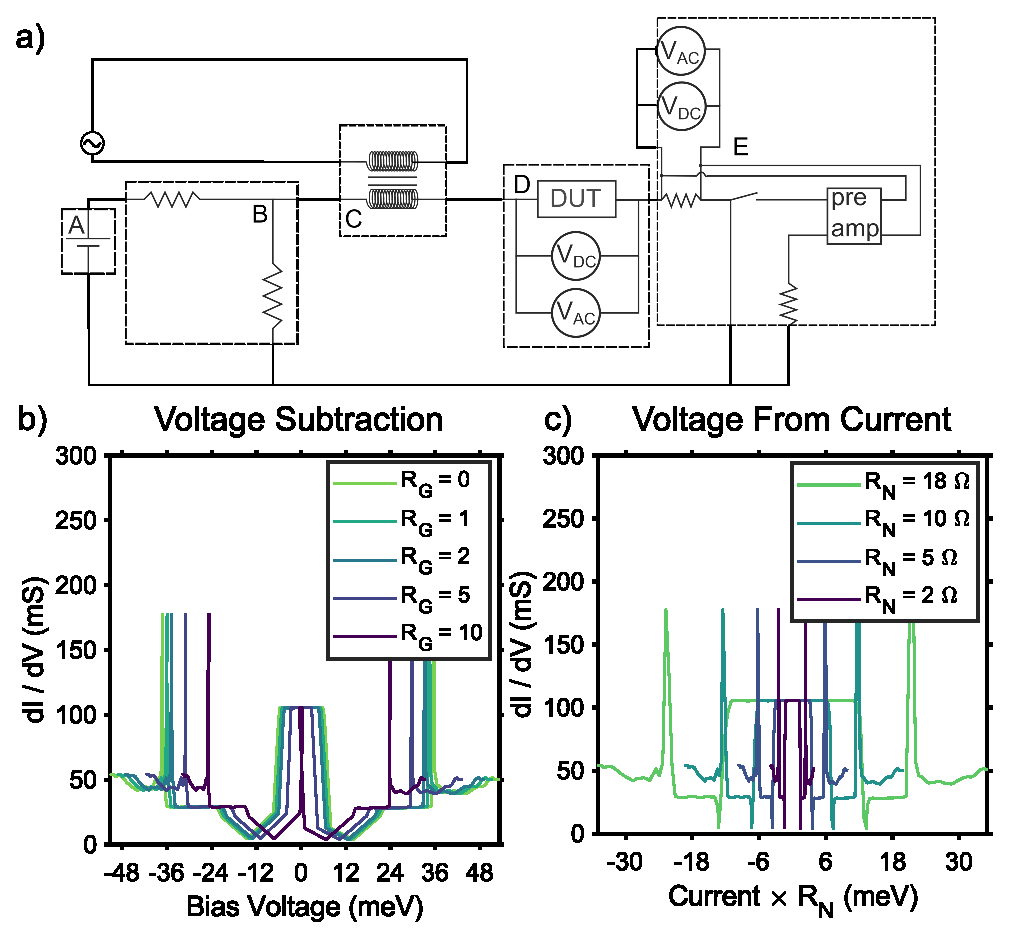
\includegraphics{Appendices/Figures/Circuit.eps}
    \caption{a) Circuit diagram to add AC and DC voltages then measure differential conductance as a function of applied DC bias. b) Voltage correction of data in Chapter \ref{chap:PAR} via subtraction of extra measured voltage due to the system resistances along the way. c) Voltage correction of the same data by measuring the resulting current and multiplying it by the normal resistance.}
    \label{fig:Circuit}
\end{figure}

\subsection{Circuit troubles and solutions}
The SR-570 Low Noise Current Preamplifier was found to send out a large voltage spike ($\sim$ 1V!) across the circuit when switching sensitivities, which often damaged or destroyed the device. For this reason we switched to using the resistor method. For higher resistance devices in which a pre-amp is needed to measure a much smaller current it is recommended that the user ground the device, disconnect the pre-amp, make the gain and sensitivity adjustments, then reconnect and unground the device. This is a slow process but it will ensure the pre-amp voltage spike does not damage the device under test.\par
The governing physics behind the voltage divider is shown in the equation,
\begin{align}
    V_{out} = V_{in}*\frac{R_{2}}{R_{1}+R_{2}}
\end{align}
however this model assumes that the output voltage is over an open circuit meaning that the resistance of the sample is large compared to $R_{2}$. When samples have a small resistance, the output voltage can change drastically from the expected value. This is especially concerning when the resistance of a sample changes drastically over a single measurement as can be the case when measuring superconducting tunneling. One solution is to use commercial voltage regulators to ensure a steady voltage is maintained even at high currents. However, most of these commercial voltage regulators have a minimum voltage output around 1.2 V which is three orders of magnitude larger than our 1 mV resolution requirement. Another solution is to switch to current-biased measurements when dealing with low-resistance samples however converting back to bias voltage can be quite tricky as will be discussed in the next section. Lastly would be to simply use a commercial high-resolution DC voltage source such as the DC205 DC Voltage Source from SRS in order to eliminate the voltage divider completely. These sources can be quite expensive but offer resolutions down to the $\mu$V level.\par 

\section{Three-point measurements}
Lastly, I would like to discuss some peculiarities with the three-point measurements used in Chapters III \& IV. In particular, since we use the measured voltage across the junction as our bias voltage (independent axis) we need to carefully consider what voltage is actually being applied across the relevant part of the junction. To illustrate, the reason a four-probe (Kelvin) measurement is preferred when determining a sample's resistivity is the Kelvin resistance does not include contact resistance\cite{Kuphaldt2015}. However in our measurement the quantity that we are measuring \textit{is} the contact resistance thus we want to be sure we don't split that resistance out of our measurement. This presents an issue as the resistance of the chrome/gold contacts will also stay in the measurement and add additional voltage to our bias voltage reading. There are two ways to correct for this: 1) Use the resistivity of a control chrome/gold device to subtract out the resistance (and voltage) or 2) convert the measured current back to a voltage by multiplying by the normal state resistance of the junction. The results of both correct are shown below for varying values of gold resistance.